% Options for packages loaded elsewhere
\PassOptionsToPackage{unicode}{hyperref}
\PassOptionsToPackage{hyphens}{url}
%
\documentclass[
  ignorenonframetext,
]{beamer}
\usepackage{pgfpages}
\setbeamertemplate{caption}[numbered]
\setbeamertemplate{caption label separator}{: }
\setbeamercolor{caption name}{fg=normal text.fg}
\beamertemplatenavigationsymbolsempty
% Prevent slide breaks in the middle of a paragraph
\widowpenalties 1 10000
\raggedbottom
\setbeamertemplate{part page}{
  \centering
  \begin{beamercolorbox}[sep=16pt,center]{part title}
    \usebeamerfont{part title}\insertpart\par
  \end{beamercolorbox}
}
\setbeamertemplate{section page}{
  \centering
  \begin{beamercolorbox}[sep=12pt,center]{part title}
    \usebeamerfont{section title}\insertsection\par
  \end{beamercolorbox}
}
\setbeamertemplate{subsection page}{
  \centering
  \begin{beamercolorbox}[sep=8pt,center]{part title}
    \usebeamerfont{subsection title}\insertsubsection\par
  \end{beamercolorbox}
}
\AtBeginPart{
  \frame{\partpage}
}
\AtBeginSection{
  \ifbibliography
  \else
    \frame{\sectionpage}
  \fi
}
\AtBeginSubsection{
  \frame{\subsectionpage}
}
\usepackage{lmodern}
\usepackage{amssymb,amsmath}
\usepackage{ifxetex,ifluatex}
\ifnum 0\ifxetex 1\fi\ifluatex 1\fi=0 % if pdftex
  \usepackage[T1]{fontenc}
  \usepackage[utf8]{inputenc}
  \usepackage{textcomp} % provide euro and other symbols
\else % if luatex or xetex
  \usepackage{unicode-math}
  \defaultfontfeatures{Scale=MatchLowercase}
  \defaultfontfeatures[\rmfamily]{Ligatures=TeX,Scale=1}
\fi
\usetheme[]{Singapore}
% Use upquote if available, for straight quotes in verbatim environments
\IfFileExists{upquote.sty}{\usepackage{upquote}}{}
\IfFileExists{microtype.sty}{% use microtype if available
  \usepackage[]{microtype}
  \UseMicrotypeSet[protrusion]{basicmath} % disable protrusion for tt fonts
}{}
\makeatletter
\@ifundefined{KOMAClassName}{% if non-KOMA class
  \IfFileExists{parskip.sty}{%
    \usepackage{parskip}
  }{% else
    \setlength{\parindent}{0pt}
    \setlength{\parskip}{6pt plus 2pt minus 1pt}}
}{% if KOMA class
  \KOMAoptions{parskip=half}}
\makeatother
\usepackage{xcolor}
\IfFileExists{xurl.sty}{\usepackage{xurl}}{} % add URL line breaks if available
\IfFileExists{bookmark.sty}{\usepackage{bookmark}}{\usepackage{hyperref}}
\hypersetup{
  pdftitle={CAMS discaRd Update},
  pdfauthor={Ben Galuardi \& Dan Linden;},
  hidelinks,
  pdfcreator={LaTeX via pandoc}}
\urlstyle{same} % disable monospaced font for URLs
\newif\ifbibliography
\usepackage{graphicx,grffile}
\makeatletter
\def\maxwidth{\ifdim\Gin@nat@width>\linewidth\linewidth\else\Gin@nat@width\fi}
\def\maxheight{\ifdim\Gin@nat@height>\textheight\textheight\else\Gin@nat@height\fi}
\makeatother
% Scale images if necessary, so that they will not overflow the page
% margins by default, and it is still possible to overwrite the defaults
% using explicit options in \includegraphics[width, height, ...]{}
\setkeys{Gin}{width=\maxwidth,height=\maxheight,keepaspectratio}
% Set default figure placement to htbp
\makeatletter
\def\fps@figure{htbp}
\makeatother
\setlength{\emergencystretch}{3em} % prevent overfull lines
\providecommand{\tightlist}{%
  \setlength{\itemsep}{0pt}\setlength{\parskip}{0pt}}
\setcounter{secnumdepth}{-\maxdimen} % remove section numbering

\title{CAMS discaRd Update}
\author{Ben Galuardi \& Dan Linden \and \footnote<.->{APSD}}
\date{2021-03-23}

\begin{document}
\frame{\titlepage}

\begin{frame}{Discard Rate Current Method Summary (J. Michael Lanning
summary)}
\protect\hypertarget{discard-rate-current-method-summary-j.-michael-lanning-summary}{}

\begin{enumerate}
\tightlist
\item
  Rates determine by observer reported values (gear, area, etc)
\item
  Incomplete observed trips have missing `hauls' prorated by observed
  information from that trip
\item
  Trips with observer get reported/calculated observed discards of that
  specific trip
\item
  Unobserved trips get discards from the rate calculated from 1)
\item
  QM is only interested in the summary total of discards for each trip,
  not subtrips. Often the interested number is a summary of trips, ie.
  the herring total of bycatch for an area/season or a sector's season's
  total of GB Cod.
\item
  Other others are driven by regs. Here I would place transition rates
  and EM methods.
\end{enumerate}

\end{frame}

\begin{frame}{discaRd Base and Support tables}
\protect\hypertarget{discard-base-and-support-tables}{}

\begin{figure}
\centering
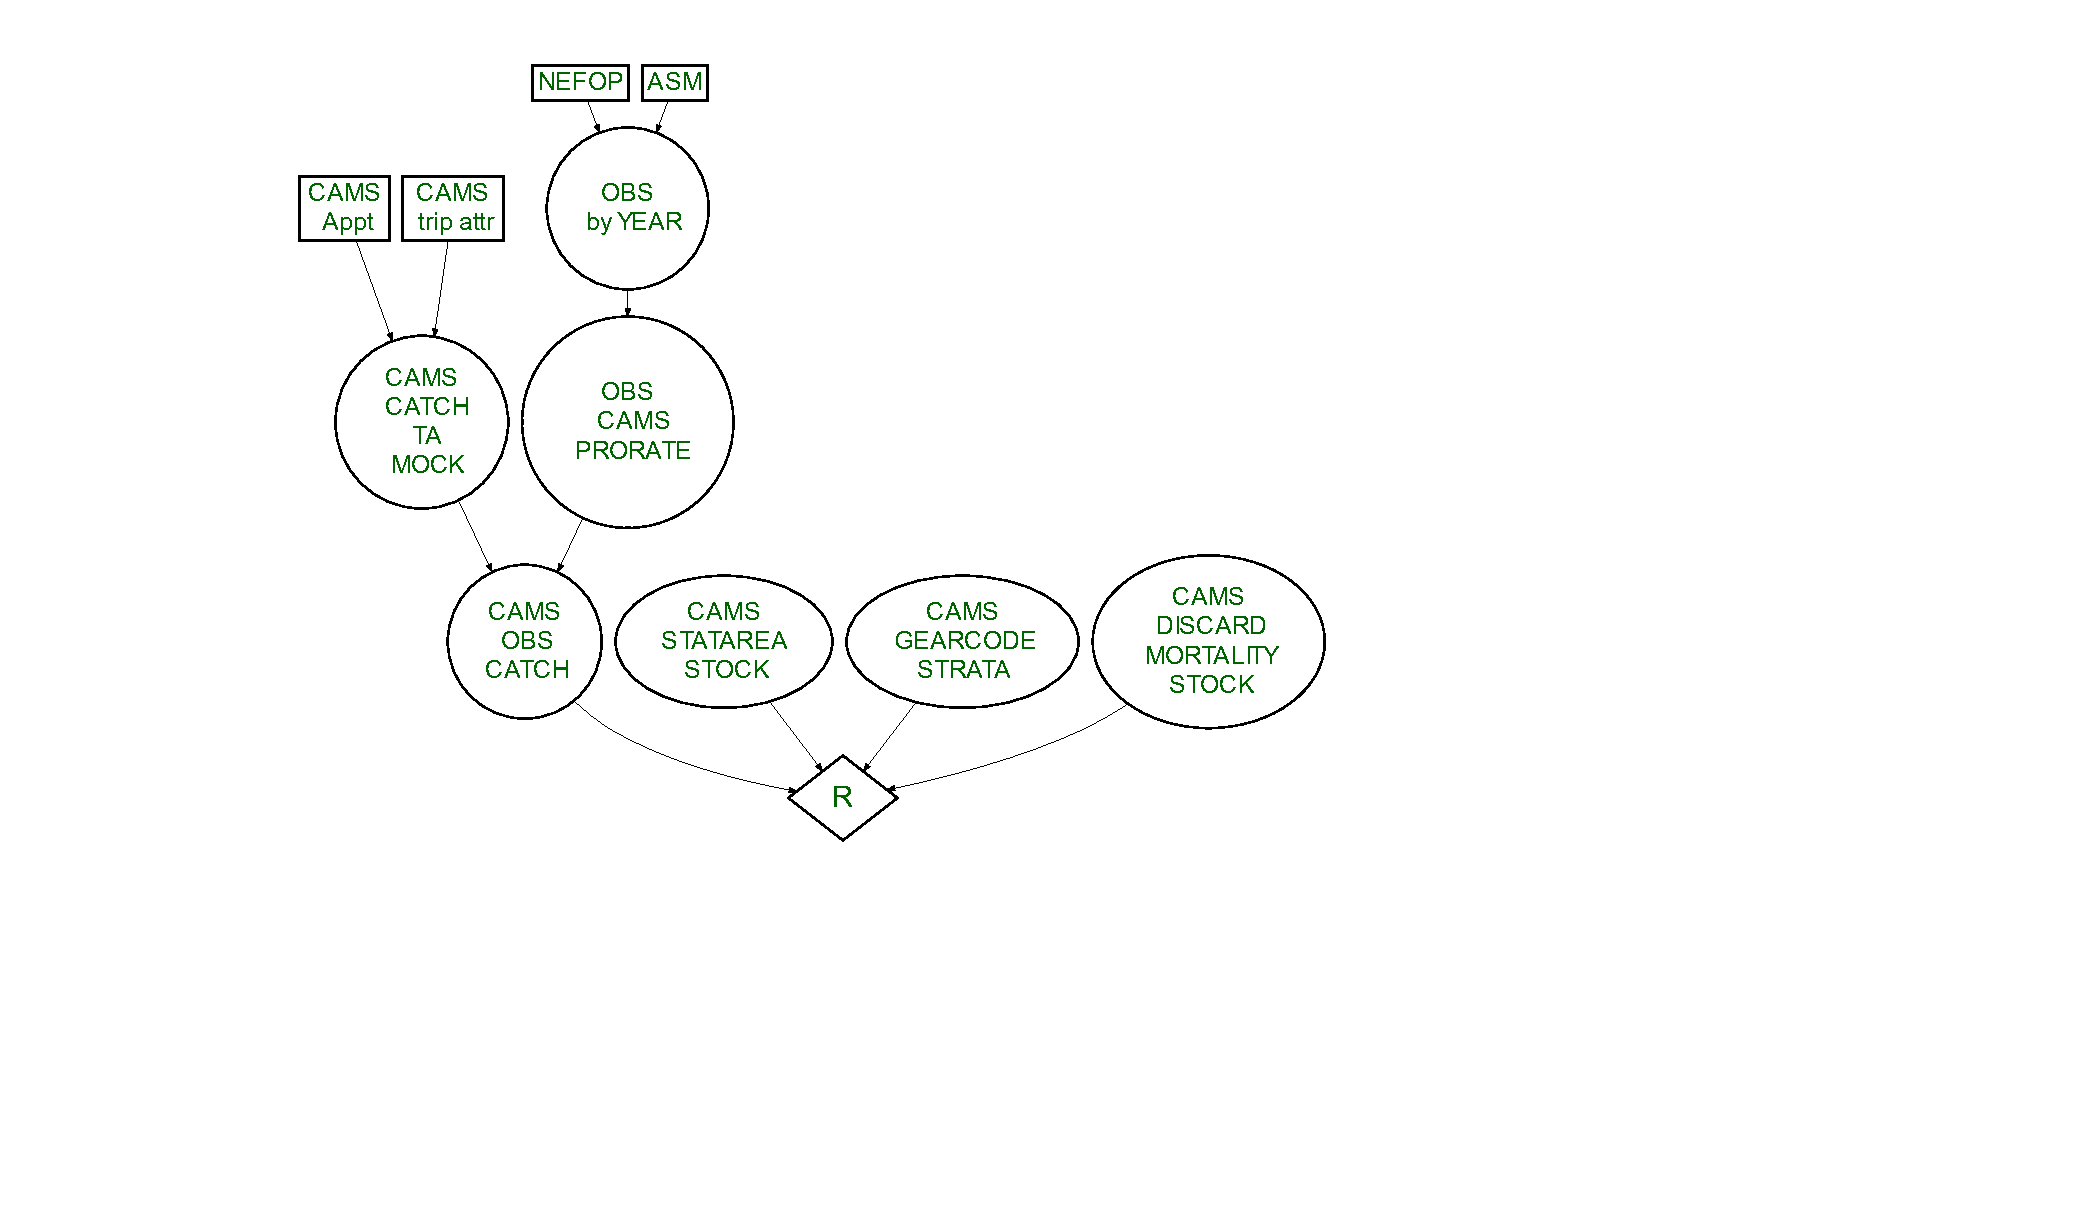
\includegraphics{discard_documention_beamer_files/figure-beamer/table_flow0-1.pdf}
\caption{Base tables (rectangle), Intermediary (circle), and Support
tables (Oval)}
\end{figure}

\end{frame}

\begin{frame}{Prorated discards}
\protect\hypertarget{prorated-discards}{}

\textbf{Incomplete observed trips have missing `hauls' prorated by
observed information from that trip}

Prorate observed discards on unobserved hauls within a subtrip. This is
done by applying a ratio of kept all on the entire trip to kept all on
the unobserved hauls only

\[d_{total} = d_{observedhauls}*(1+KALL_{unobserved hauls}/KALL_{subtrip})\]

\end{frame}

\begin{frame}[fragile]{R Process}
\protect\hypertarget{r-process}{}

\texttt{discaRd} R package built for 2016 Discard Estimation Peer Review


\includegraphics[width = .25\textwidth, height = .25\textheight]{discaRd.png}

New functions for CAMS:

\begin{itemize}
\tightlist
\item
  \texttt{make\_assumed\_rate} Calculates `fallback rate' using a subset
  of \texttt{STRATA} variables
\item
  \texttt{make\_bdat\_focal} Constructs data frame of observed trip data
  for species of interest
\item
  \texttt{run\_discard} Runs these functions in conjucntion with
  \texttt{discaRd}
\end{itemize}

\end{frame}

\begin{frame}[fragile]{Running it}
\protect\hypertarget{running-it}{}

\begin{itemize}
\tightlist
\item
  refresh Oracle tables?
\item
  define species and stock (if applicable)

  \begin{itemize}
  \tightlist
  \item
    generates SQL
  \end{itemize}
\item
  import to R

  \begin{itemize}
  \tightlist
  \item
    apply CAMS\_GEAR\_GROUP according to SPECIES
  \item
    apply STOCK STAT AREA according to SPECIES and stock (if needed)
  \item
    join discard mortality by species/stock/CAMS\_GEAR\_GROUP
  \end{itemize}
\item
  \texttt{run\_discard}

  \begin{itemize}
  \tightlist
  \item
    STRATA is assigned dynamically by using elements of the imported
    data
  \item
    If using \texttt{transition\ rates}, two time periods are defined
  \item
    Assumed (fallback rates) are defined as a subset of STRATA
  \end{itemize}
\item
  Apply Discard Mortality
\end{itemize}

\end{frame}

\begin{frame}[fragile]{TO DO}
\protect\hypertarget{to-do}{}

\begin{itemize}
\tightlist
\item
  utilize support tables

  \begin{itemize}
  \tightlist
  \item
    \texttt{CAMS\_GEAR\_GROUP} \textbf{DONE}
  \item
    \texttt{STAT\_AREAS} \textbf{DONE}
  \item
    \texttt{CAMS\_DISCARD\_MORTALITY\_STOCK} \textbf{in process}
  \end{itemize}
\item
  add \texttt{SECTOR} for multispecies (see above) \textbf{DONE}
\item
  Time periods \textbf{Determined by STOCK/SPECIES}

  \begin{itemize}
  \tightlist
  \item
    Species with the same time period, e.g.~Calendar year, can be
    imported at once.
  \end{itemize}
\item
  Assumed (fallback) rate criteria: how simplified must this be?
\item
  implement transitions (if using fixed time period) \textbf{DONE}
\item
  Deal with Exemptions
\item
  Incorporate stratification for EM trips
\item
  refine exact operational process*
\end{itemize}

*\textbf{Will likely be based on modules that run common sets of species
(e.g.~common \texttt{CAMS\_GEAR\_GROUP} and stock definition)}

\end{frame}

\begin{frame}{Modules}
\protect\hypertarget{modules}{}

\begin{itemize}
\tightlist
\item
  Quota Monitoring

  \begin{itemize}
  \tightlist
  \item
    Squid/Mackerel/Butterfish (Calendar year) ++ This may encompass any
    UNIT stock with calendar year
  \item
    Groundfish (May year)
  \item
    Monkfish (May year)
  \item
    Yellowtail/Windowpane in scallop fishery (April year)
  \item
    Skates (?)
  \item
    Small mesh species (hakes)
  \item
    ??
  \end{itemize}
\item
  SBRM

  \begin{itemize}
  \tightlist
  \item
    300 species on SBRM year (Calendar?) -Stock Assessments
  \item
    typically run on calendar years for all species
  \end{itemize}
\end{itemize}

\end{frame}

\end{document}
